\documentclass[10pt]{article}
\usepackage{url}
\usepackage{a4}
\usepackage{alltt}
\usepackage{epsfig}

\setlength{\parindent}{0pt}
\setlength{\parskip}{4pt}

\pagestyle{empty}

\author{Armijn Hemel}
\title{Universal Plug and Play: Dead simple or simply deadly?}

\begin{document}

\maketitle
\thispagestyle{empty}

\section{Universal Plug and Play overview}

Many devices and programs that exist today have support for the Universal
Plug and Play (UPnP) protocol. The UPnP protocol emerged from within
Microsoft in early 1999 to bring the plug and play concept as found on
Windows desktop machines to the local network. The idea behind UPnP is to
enable a user to plug a device into the local network and it will simply
work, whether the device is a printer, scanner, fileserver or firewall.
All configuration is hidden for the user and instead done automatically by
the devices and programs themselves.

The first implementations of UPnP were shipped halfway 2000, Windows
ME and Intel's open source UPnP SDK for Linux being the first. Windows XP also had UPnP
support built-in since its release in 2001. There are currently
implementations for various operating systems, including Windows, VxWorks,
Linux\cite{libupnp}\cite{linux-igd} and FreeBSD\cite{libupnp}\cite{linux-igd}.
The UPnP protocol stack uses well-defined Internet standards, such as HTTP,
XML and SOAP.

One of the best known programs that uses UPnP is Microsoft's MSN Messenger.
Ports that need to be opened on the firewall for voice and video traffic
(the ``webcam'' feature) and direct file transfers in MSN Messenger are
allocated dynamically using UPnP. This is done by sending special UPnP commands
to a UPnP enabled firewall if the machine that runs MSN Messenger is behind
a firewall or NAT device and cannot communicate with the other machine
directly. These commands instruct the firewall to forward ports on the
firewall's external interface to ports that MSN Messenger uses on on the
machine on the inside network.

Other programs that use UPnP to open up ports in firewalls are networked
games. Online gaming networks, like Microsoft's X-Box Live, also heavily
rely on UPnP.

Another use is Voice over IP (VoIP). The most frequently used open VoIP
protocols (H323, SIP) have a rather complex flow of network packets with
multiple packet streams flowing back and forth. For example, the SIP protocol
stack uses a few different protocols during the duration of a phonecall. First
a connection is set up between two machines using SIP to negotiate various
properties of the connection, such as the codec which has to be used. If this
negotiation is successful a new connection is set up between the
machines in both directions using RTP. The port for the incoming traffic
should be opened in the firewall, otherwise the communication will be one-way,
because RTP packets will simply be dropped\footnote{And even then it is not
guaranteed to work. The RTP protocol encodes the IP address inside the TCP
payload. A normal NAT device will not rewrite the IP address inside the RTP
packet. To do this you will need a special proxy NAT device that knows
how to rewrite RTP packets properly.}. With UPnP the incoming port on the
firewall could be opened in advance, or opened once the SIP negotiation has ended
and before the RTP streams are set up. There are several phones with built-in
support for UPnP, for example, the snom220 phone (which is no longer
available), although for phones other NAT traversal mechanisms seem to be
more popular these days.

An advantage of using UPnP is that there does not have to be a predefined
well-known port for every protocol. It allows for multiple simultanious
connections for the same program by different users. With dynamically allocated
ports user A uses different ports on the firewall than user B for the same
protocol. Ports can be closed again after usage by the program or device
itself, so there should be no resource hogging.


\section{Universal Plug and Play protocol flaws}

While UPnP is convenient from a user point of view -- programs that need to
dynamically have ports allocated or need special ports on the firewall to
be forwarded to them to work correctly can do this automatically -- there is,
unfortunately, a price to pay. As it is defined in the current standard, UPnP
has no default security mechanism. There is add-on functionality which adds
security but devices that implement this functionality are very scarce, if
they even exist beyond the prototype stage.

With the current UPnP protocol there is an implicit trust relationship
between all UPnP capable devices on the same network. Every device is a peer
and there is no policy mechanism in place to check whether or not a device is
allowed to make use of a specific service.

A few simple scripts that implement only a small subset of commands that are
used in UPnP are enough in certain situations to make it possible to expose
machines and services on an internal network to the outside world. This is
done by abusing a device that implements the UPnP Internet Gateway Device
profile and forward ports on the outside interface of the Internet Gateway
Device to machines on the inside network. This makes the internal machine
accessible for everyone on the outside network, for example the Internet.
Many ADSL routers and wireless access points on the market nowadays implement
this particular profile and of those devices many are, in various ways,
vulnerable to various ``attacks''.

The UPnP Internet Gateway Device specifications specifically mention that
it should be possible to forward ports to internal multicast and broadcast
addresses, so devices can share broadcast/multicast streams, for example a
TV stream. The benefit for the sender and receiver is that only one stream
has to be sent to the gateway, which will resend it to the LAN so it can be
shared between machines on the LAN, saving bandwidth. But forwarding ports
to broadcast addresses also opens up a whole new range of attacks. To name
two possible targets: the NetBIOS Naming Service used by Windows network file
sharing and the Internet Printing Protocol, used by many printers and CUPS,
both use broadcasting. It is trivial to announce fake printers on the network
and possibly divert printing traffic to off site printers.

Opening and forwarding ports in firewalls via UPnP poses a serious threat.
While at first this might seem to only affect home users and not businesses
-- no enterprise range products seem to support UPnP -- I tend to think
otherwise. It could very well affect business users as well, for a number of
reasons:

\begin{itemize}
\item Many (small) businesses are connected via normal ``consumer grade'' ADSL
lines and have the same ADSL modem as normal home users. For a long time the
default Ethernet ADSL modem that was used by KPN in the Netherlands was the
Alcatel/Thomson Speedtouch 510, which enables UPnP by default. In the web
interface of this device there is no possibility to disable UPnP. Users have
to use the commandline interface to shut off UPnP, which is beyond the
technical capability of many users.

\item Wireless access points and routers that are primarily meant for home
use are also frequently used inside (small) company networks (``SOHO'').
The Linksys brand of access points and routers is especially popular in
this segment of the market. War driving has shown that many administrators do not
properly configure wireless access points and routers, which makes it likely
that UPnP is also enabled on those networks.

\item Many, if not most, attacks on company networks originate from normal
consumer lines (``zombie networks'' come to mind). The fact that millions of
UPnP enabled routers were sold makes this something that should not be
ignored.

\end{itemize}

A threat to businesses is that services that should not be exposed to the
outside, such as internal DNS or NFS/SMB file servers can now easily be opened
up to the whole world. These fileservers often contain sensitive and important
information.

A firewall cannot be trusted to keep out the bad guys anymore (even though
relying on just a firewall is bad anyway), making it as likely to be hacked
as when the machine is hooked up to the Internet directly. Having good host
security is (and always has been) important and is often overlooked.

So far it seems that there has been not much research in the area of abusing
the port mapping feature of UPnP Internet gateway devices. It could be that
many people do not see it as a threat, or that this hack is simply too obvious
that no one thinks it is good enough to exploit it. However, many of the most
effective cracks are done via simple holes. My hopes are that this paper
can somehow fuel the discussion for integrated security in SOHO and
home user networking equipment.


\section{Design of UPnP}

The UPnP protocols are developed by the UPnP Forum\cite{upnpforum}, the
UPnP standardization committee. It oversees the development of new profiles
and standards. In this section I will give a short description of how UPnP is
designed. A more thorough description can be found in the book ``UPnP: Design
by Example''\cite{intel}.

\subsection{Profiles}

Central to the concept of UPnP are profiles. A machine or a piece of software
can implement one or more profiles and provide services accordingly. The UPnP
Forum has defined various default profiles, including profiles for printers,
HVAC (Heating, Ventilating, and Air-Conditioning) systems and so on. The first
profile that was certified was the Internet Gateway Device profile. Devices
which implement the Internet Gateway Device profile are meant to provide
access to WLAN connections, such as the Internet. Devices that implement the
Internet Gateway Device profile are routers, wireless access points and ADSL
modems. In this paper the focus will be on devices that implement this profile.

In the UPnP documentation devices that can provide a service are called
``control points''. Machines or programs that make use of these control
points are referred to as ``devices''. The role a machine has can be
different per context. For example, a machine that is normally a ``control
point'' (for example a file server) can be a ``device'' if it needs to have
ports opened up in the firewall dynamically. The terms that are used in UPnP
documentation are a bit ambiguous.

A control point can implement more than one profile. Many profiles only
serve as containers for other profiles, or as an abstraction for other
profiles, similar to interfaces or abstract classes in object oriented
programming languages. These profiles are commonly called ``subprofiles''.
The Internet Gateway Device profile is a container for a few other profiles.
It is mandatory for the Internet Gateway Device profile to implement 
\texttt{WANDevice}, which in turn has to have at least one
\texttt{WANConnection}. A control point which implements Internet Gateway
Device can also implement other subprofiles, such as LANDevice.

The WANConnection profile is an example of an abstraction. It is never
directly implemented itself, but it is ``instantiated'' by implementing
\texttt{WANPPPConnection}, which is often used for DSL routers,
or \texttt{WANIPConnection}, common for normal routers or wireless
gateways.


\subsection{Protocol design}

In UPnP there are a few steps that every device goes through, or can go
through. Some of these steps are mandatory, others are used depending on
what role a device has.

\subsubsection{Step 0: Addressing}

The first (or actually, zeroth) step in UPnP is addressing. This step is
performed when a device is connected to a network. If it cannot obtain an IP
address via DHCP, because a DHCP server is absent, it will assign an IP
address to itself and try to determine if the IP address is unused. The
address is chosen from the \texttt{169.254/16} range. If the address is in
use, the device will try to assign another IP address until it has obtained
an IP address that it can use. This is often called ``auto-addressing''. The
underlying thought is that this way devices can organise the network
themselves without having to rely on a central control point, like a DHCP
server, or a system administrator that assigns IP addresses.

This ``auto-addressing'' technique is not unique to UPnP. Other protocols,
such as IETF ZeroConf, use similar techniques. Some Linux distributions,
like Fedora Core 3 and Fedora Core 4, also include default routes for the
\texttt{169.254/16} network in their network configuration.

Even in a network which uses a DHCP server some UPnP devices will sometimes
still send packets using one of the IP addresses in the \texttt{169.254/16}
range. The Alcatel Speedtouch 510 ADSL router sends UPnP notification messages
(see step 1) using an IP address in this range.


\subsubsection{Step 1: Discovery}

When a machine joins a network and wants to know what UPnP services are
available on the network, it sends out a discovery message to
\url{239.255.255.250} on port 1900 via UDP. This message contains a header,
similar to a HTTP request:

\begin{verbatim}
M-SEARCH * HTTP/1.1
HOST: 239.255.255.250:1900
MAN: ssdp:discover
MX: 10
ST: ssdp:all
\end{verbatim}

All control points are required to respond to this message by sending back a
similar message via UDP unicasting back to the device, announcing which UPnP
profiles the control point implements. For every profile it implements one
message is sent:

\begin{verbatim}
HTTP/1.1 200 OK
CACHE-CONTROL:max-age=1800
EXT:
LOCATION:http://10.0.0.138:80/IGD.xml
SERVER:SpeedTouch 510 4.0.0.9.0 UPnP/1.0 (DG233B00011961)
ST:urn:schemas-upnp-org:service:WANPPPConnection:1
USN:uuid:UPnP-SpeedTouch510::urn:schemas-upnp-org:service:WANPPPConnection:1
\end{verbatim}

The above is a slightly edited response that is sent by an Alcatel/Thomson
Speedtouch ADSL modem. Some implementations of the UPnP stack do not seem to
send responses back at all.

The response message contains a header called \texttt{LOCATION}, which
is a URL where a file in XML format can be downloaded which describes the
services that the control point implements. There is no default location for
this file. In some control points, such as the OvisLink MU-5000FS, a
Linux/Samba based network storage device (also available from other vendors),
the \texttt{LOCATION} header even differs between reboots as the port on
where the webserver runs is dynamically assigned.

At a regular interval control points have to send a message to announce
their services. A notification message is the same as a response message to
a discovery, but they are sent to the UPnP broadcast address
(\url{239.255.255.250}) on port 1900 via UDP.

Also, the header \texttt{ST} is replaced by the header \texttt{NT}, but with
similar values.

\subsubsection{Step 2: Description}

Every profile offers a description of itself and the services it offers
and makes this available via XML. The XML file can be found at the
URL in the \texttt{LOCATION} header from the discovery stage.

\subsubsection{Step 3: Control}

The third step in the protocol is called ``control'', which means that a
device can ask a control point to request a service on the client's behalf.
Requesting a service is done by sending a SOAP request to the so called
``control URL'' of the control point, with the right parameters. The control
URL for a specific profile can be found inside the \texttt{<service>} tag in
the XML file found at the URL in the \texttt{LOCATION} header. As an example
the \texttt{<service>} tag from the Thomson Speedtouch 510 for the
\texttt{WANPPPConnection} profile looks like this:

\begin{verbatim}
<service>
  <serviceType>urn:schemas-upnp-org:service:WANPPPConnection:1</serviceType>
  <serviceId>urn:upnp-org:serviceId:wanpppc:pppoa</serviceId>
  <controlURL>/upnp/control/wanpppcpppoa</controlURL>
  <eventSubURL>/upnp/event/wanpppcpppoa</eventSubURL>
  <SCPDURL>/WANPPPConnection.xml</SCPDURL>
</service>
\end{verbatim}

For sending SOAP requests only \texttt{controlURL} is necessary. The
\texttt{eventSubURL} is used in the next step. Which actions can be performed
depends on the profile. The URL found at \texttt{SCPDURL} is the so called
``URL for service description'' and it describes which SOAP requests can
be performed and what the so-called state variables are.

SOAP is a protocol that runs over HTTP and uses XML to describe ``function
calls'' to a server and return results from those calls. SOAP is mainly used to
make use of web based services. For every major programming language 
libraries are available that can be used to implement SOAP requests and process
SOAP responses. Throughout this paper there are various Python code snippets.
The SOAP library that is used is SOAPpy\cite{soappy}.

One of the actions that can be performed on a control point that implements
the \texttt{WANPPPConnection} profile is \texttt{GetExternalIPAddress}, which
is used to get the external IP address of the device:

\begin{alltt}
#!/usr/bin/python

import os
from SOAPpy import *

## "endpoint" is the control URL for WANPPPConnection on a Speedtouch 510

endpoint = "http://10.0.0.138/upnp/control/wanpppcpppoa"
namespace = "urn:schemas-upnp-org:service:WANPPPConnection:1"
soapaction = "urn:schemas-upnp-org:service:WANPPPConnection:1#GetExternalIPAddress"

server = SOAPProxy(endpoint, namespace)

print "external IP", server._sa(soapaction).GetExternalIPAddress()
\end{alltt}

Adding a port mapping for the machine located at the IP address
\url{10.0.0.151} can be done with the following code:

\begin{verbatim}
soapaction2 = "urn:schemas-upnp-org:service:WANPPPConnection:1#AddPortMapping"

server._sa(soapaction2).AddPortMapping(NewRemoteHost="",
           NewExternalPort=8080,
           NewProtocol="TCP",
           NewInternalPort=80,
           NewInternalClient="10.0.0.151",
           NewEnabled=1,
           NewPortMappingDescription="internal webserver",
           NewLeaseDuration=0)
\end{verbatim}

A portmapping can be deleted with a similar SOAP action:

\begin{verbatim}
soapaction3 = "urn:schemas-upnp-org:service:WANPPPConnection:1#DeletePortMapping"

server._sa(soapaction3).DeletePortMapping(NewRemoteHost="",
           NewExternalPort=5666,
           NewProtocol="TCP")
\end{verbatim}


\subsubsection{Step 4: Eventing}

Control points keep state, which devices can read out. A device can register
with the control point to receive event messages whenever the value of a
so called state variable has changed. It does so by sending a request to the
control point:

\begin{verbatim}
SUBSCRIBE /upnp/event/wanpppcpppoa HTTP/1.1
Host: 10.0.0.138
Callback: <http://10.0.0.150:5000/notify>
Timeout: Second-1800
NT: upnp:event
\end{verbatim}

After a device has registered with a control point it will first receive
a message with the current state of all evented messages and it will receive
updates whenever the state of a variable changes. These messages will be
sent to all the URLs that are present in the \texttt{Callback} header.

\subsubsection{Step 5: Presentation}

Presentation is about how a device ``presents'' itself to normal human beings.
It nearly always comes down to being able to control the UPnP device via a
webinterface.


\section{UPnP security attacks}

UPnP is not a very complex protocol, but it is far reaching, especially when
port mappings can be done via UPnP. Implementation errors of the UPnP protocol
stack in devices, and also omissions in the specifications, enable an attacker
to do quite severe things, including hijacking of network traffic, anonymous
proxying of network traffic and exposure of trusted machines to untrusted
external networks.

This section describes a range of attacks which are possible with UPnP in
general, or with specific implementations of UPnP. These attacks all originate
from within the LAN, where a user or malicious program possibly already has
full access to some or all machines in the LAN. Tunnels to the outside are
easily created in such a setup. It can be argued that because access to the
internal LAN is a prerequisite for everything described in this paper these
attacks should not be regarded as real attacks. However, I think that the
ease with which a firewall can be completely reconfigured makes it a big
enough threat:

\begin{itemize}
\item It takes no special privileges to reconfigure a UPnP-enabled firewall.
\item Changes to the firewall done via UPnP are often persistent across
reboots of the Internet Gateway Device and not always easy to remove.
\item A computer that has been taken over by a virus, spyware or cracker is
relatively easy to detect, but a reconfigured router is a lot harder to find,
especially when the router is complying with all standards it implements.
\end{itemize}


\subsection{Exposing internal machines to outside networks}

The portmapping feature described earlier is convenient if you want to have
ports forwarded to your own machine, but it can also be abused to forward
ports on the firewall to other machines. Any host on the internal network can
ask for any portmapping it desires, so the machine on \url{10.0.0.152} could
execute the following Python code to send a SOAP packet to the Internet
Gateway Device to ask for a portforward to \url{10.0.0.151}, without
\url{10.0.0.151} even knowing about it:

\begin{verbatim}
soapaction2 = "urn:schemas-upnp-org:service:WANPPPConnection:1#AddPortMapping"

server._sa(soapaction2).AddPortMapping(NewRemoteHost="",
           NewExternalPort=22,
           NewProtocol="TCP",
           NewInternalPort=22,
           NewInternalClient="10.0.0.151",
           NewEnabled=1,
           NewPortMappingDescription="ev1l h4x0r",
           NewLeaseDuration=0)
\end{verbatim}

\begin{center}
  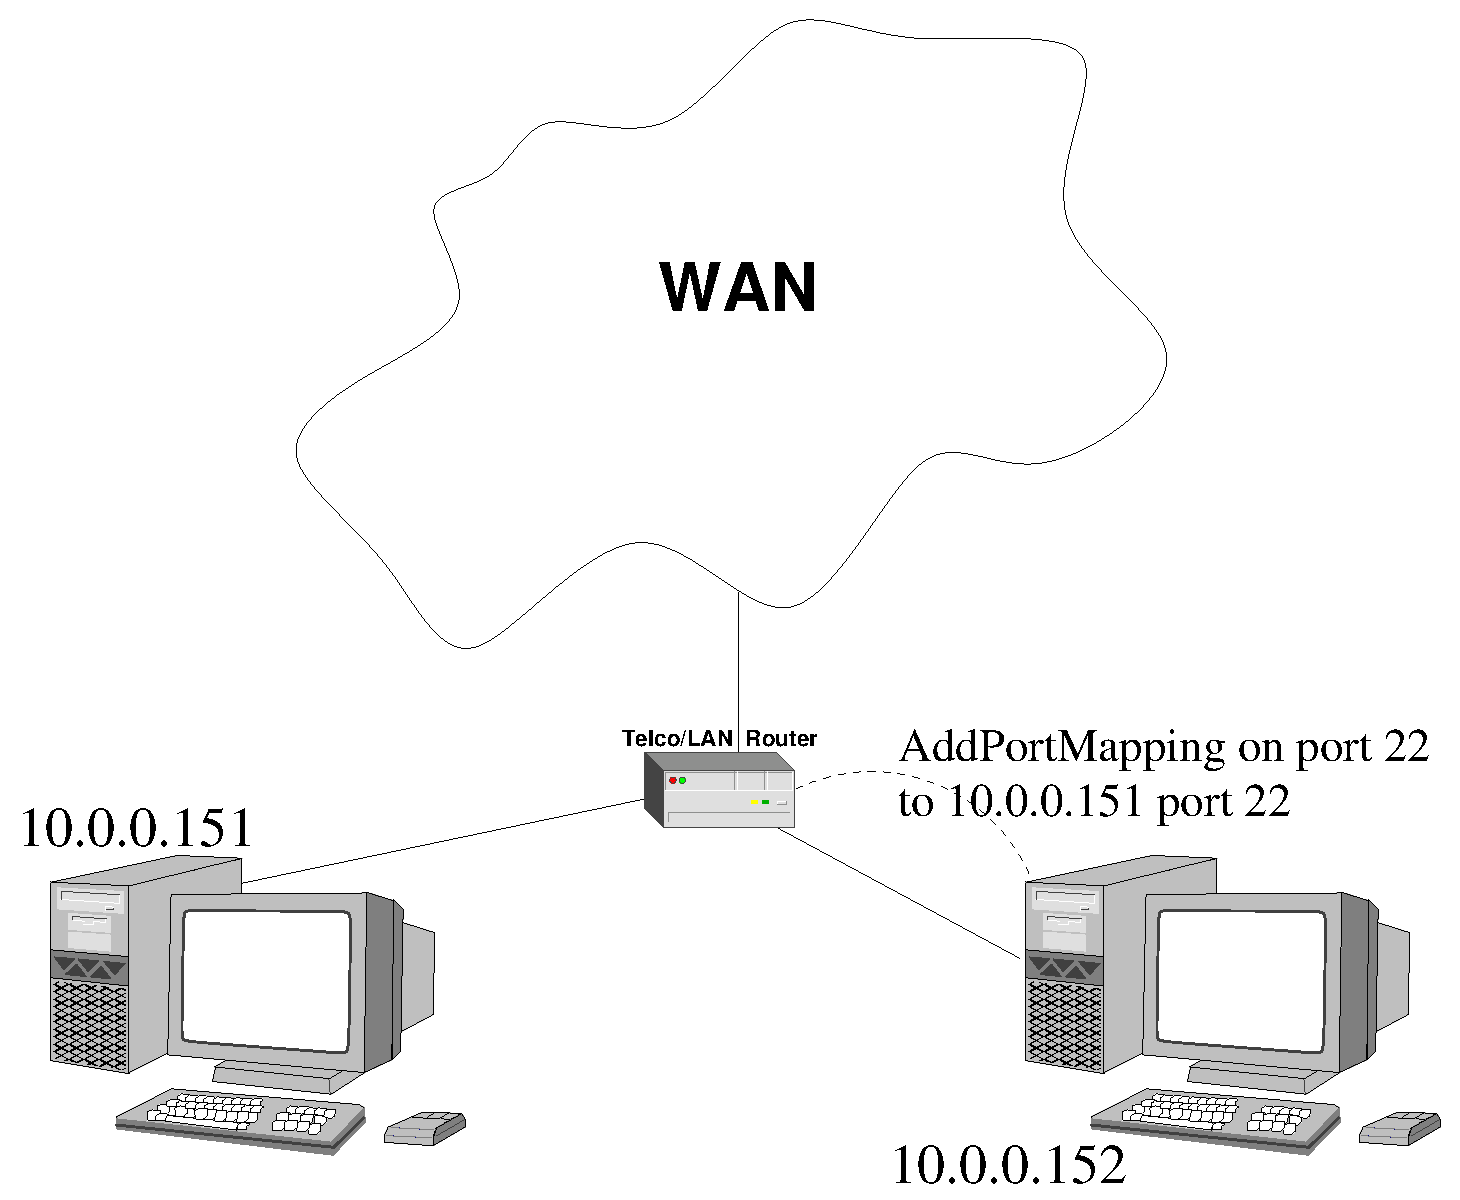
\epsfig{file=portforward2.eps, height=8cm}
\end{center}

It is up to the Internet Gateway Device to fullfill (or refuse) these
requests. Nearly all Internet Gateway Device will happily comply with such
requests.

In the specification the specifications are vague about that an Internet
Gateway Device should honour requests for portforwardings other than to the
machine that made the request.

On page 12 of the specification of the \texttt{WANIPConnection} profile
(\texttt{UPnP\_IGD\_WANIPConnection 1.0.pdf}, available from the website of
the UPnP forum\cite{upnpforum}) it says:

\begin{quote}
``This variable represents the IP address or DNS host name of an internal
client (on the residential LAN).''
\end{quote}

On page l3 of that same document it says:

\begin{quote}
``Each 8-tuple configures NAT to listen for packets on the external interface
of the WANConnectionDevice on behalf of a specific client and dynamically
forward connection requests to that client.''
\end{quote}

From the context it is not entirely clear if ``that client'' should always be
the requesting device. It should be clear that this is a security bug
and that this behaviour should explicitely be denied in the specification.

The specifications mention that it should be possible to set
\texttt{InternalClient} to \url{255.255.255.255}, a broadcasting address.

In some of the implementations (Alcatel Speedtouch 510) that were examined
this particular behaviour could be triggered.


\subsection{Using UPnP to create proxies and hijack ports}


At least one implementation of the Internet Gateway Device profile allows
anyone on the internal network to set the \texttt{InternalClient} parameter
as used by the \texttt{AddPortMapping} SOAP function to any machine on the
Internet. This implementation was developed by Broadcom for their router
platform. It can be found in certain revisions of the Linksys WRT54G(S) and
a lot of other Linux-based routers and access points (the hardware list on the
OpenWrt Wiki\cite{openwrt} gives a good indication which devices are based on
the platforms Broadcom makes).

In this particular implementation the Internet Gateway Device does not check
whether or not the \texttt{InternalClient} parameter really is a machine on
the LAN. The Internet Gateway Device, will happily perform Network Address
Translation (NAT) on the incoming packets to \texttt{InternalClient}, even if
\texttt{InternalClient} is located on an external network. The result is that
the headers of the incoming packets will be rewritten and resent from the
router.

This means that ports on the external interface of the Internet Gateway Device
can be used to forward traffic to other machines that are also on the external
interface. An attacker can exploit this bug to have his own traffic routed
through the Internet Gateway Device of the victim to masquerade his own traffic
and thus create his own onion routing system\cite{onion}\cite{tor}, but
without the permission or knowledge (logging is turned off by default) of the
owner of the router.

\subsubsection{Case: make your own onion router}

With a small bit of hacking it is possible to forward ports on the external
interface of an ADSL router, that in itself is not directly vulnerable to the
attack described above, to another host on the Internet, where it will appear
as if all traffic is coming from the ADSL router. This can be done as long as
there is some router in the network that is vulnerable.

The machines involved are:

\begin{itemize}
\item Alcatel/Thomson Speedtouch ADSL router (using PPPoA), internal IP address \texttt{10.0.0.138}
\item machine A, IP address \texttt{10.0.0.151}
\item Linksys WRT54G, external IP address \texttt{10.0.0.152} and internal
IP address \texttt{192.168.1.1}
\item machine B, IP address \texttt{192.168.1.100}
\end{itemize}

\begin{center}
  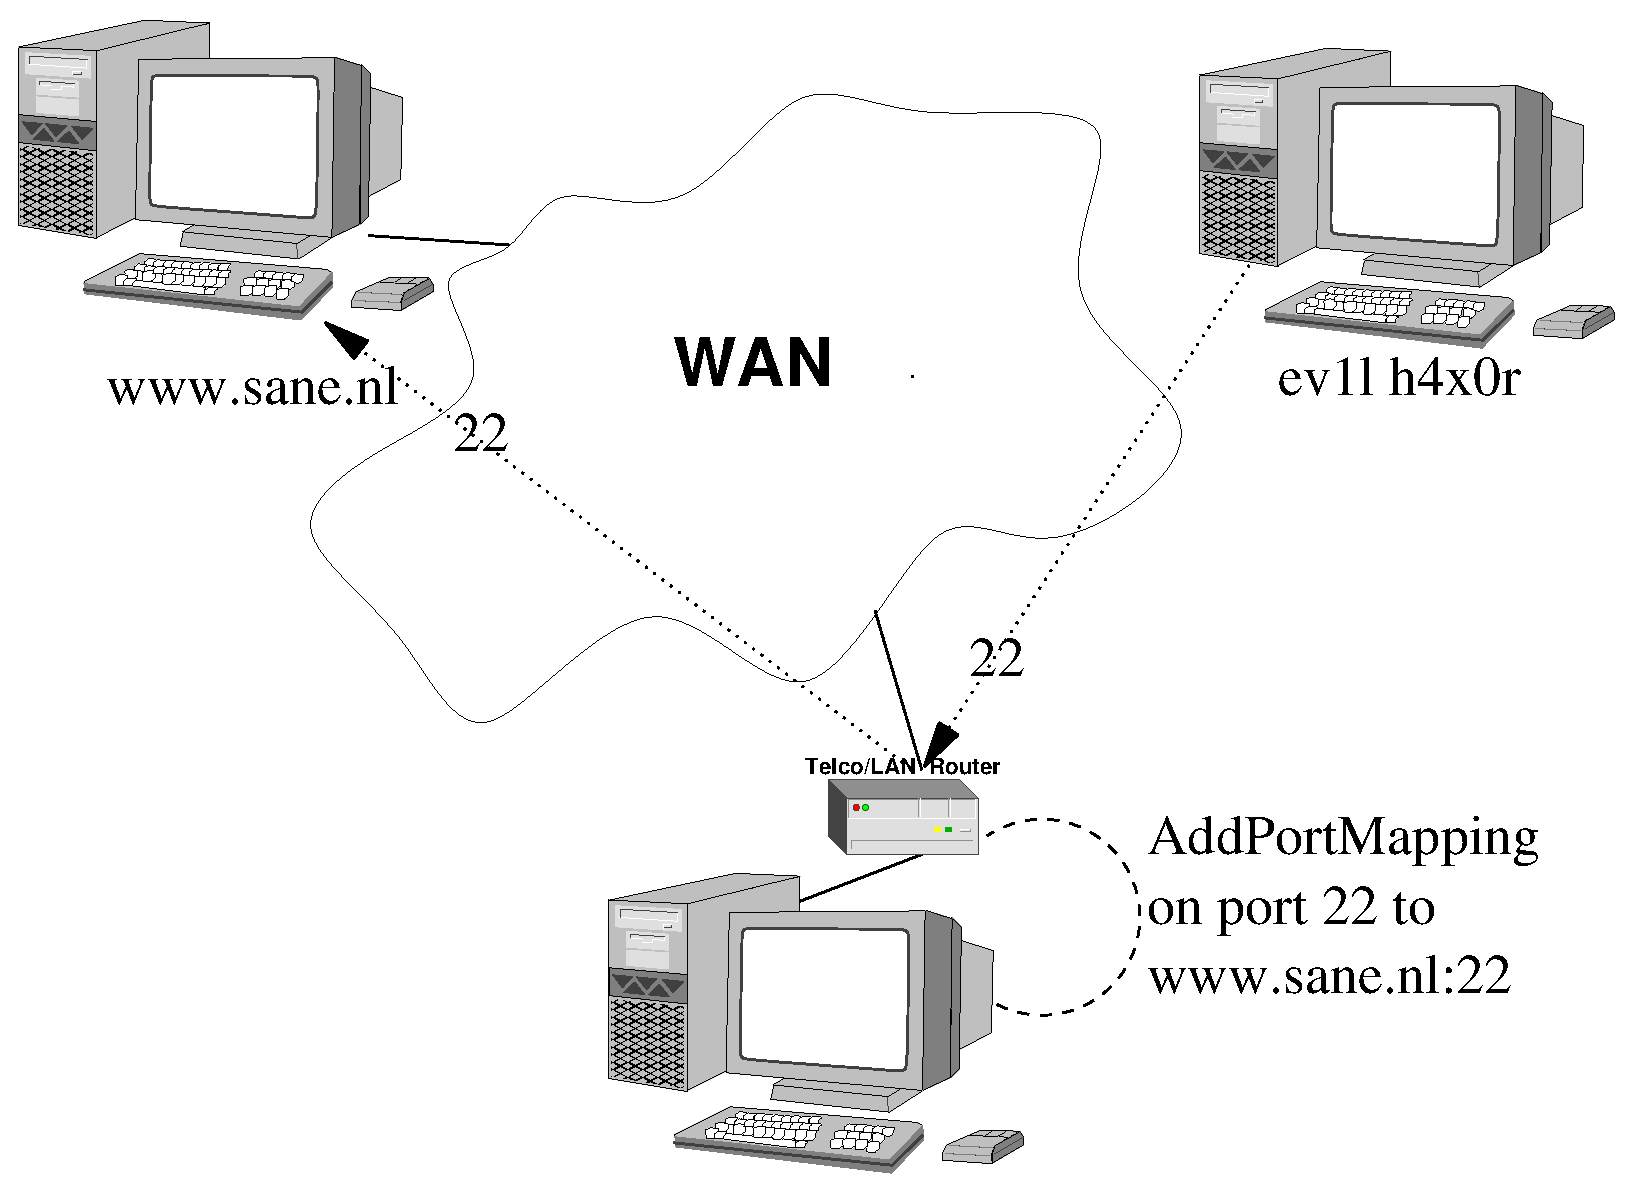
\epsfig{file=portforward.eps, height=8cm}
\end{center}


The hack works as follows:

\begin{itemize}
\item Let machine A ask the Speedtouch to forward all traffic on port 22
on the external interface to port 22 on the Linksys router.
\item Let machine B exploit the bug in the UPnP implementation on the Linksys
router and let the router forward port 22 on the external interface to port
22 on a random host on the Internet (say \url{www.sane.nl})
\end{itemize}

This way, if you connect to the ADSL router on port 22 from the Internet,
you will be routed to port 22 on \url{www.sane.nl}. Because all
traffic will go through two NAT devices (namely the Linksys WRT54G and the
ADSL router) it will appear as if all traffic comes from the ADSL router.
The hack can be made a bit simpler if machine B asks the ADSL router to make
the portforward instead of machine A.

Of course, if the only link between the Internet and the inside network
is the WRT54G, the hack is in fact a lot simpler. In the Netherlands this
situation is not very common, since the WRT54G has no built-in ADSL
modem.

More serious hacks are possible with this bug. For example, this hole could be
exploited to hijack port 25 to capture someone's mail if a mail server is
running behind the Internet Gateway Device and port 25 on the external
interface is forwarded to the internal mailserver. Hijacking can be done by
first deleting the existing portmapping for port 25 from the Internet Gateway
Device and then creating a new mapping to an external machine in the same
way as is described above.

In a similar way you could redirect port 80 to another machine, and deface
a website without having to break into the webserver, or divert traffic and
use it for phishing.

This bug was reported to Linksys in early february of 2006. Linksys found
the bug, but a replacement firmware was not yet available before the deadline
for this paper. Other vendors haven't fixed it yet. The sad truth is that this
bug apparently was already known by at least one vendor. In the GPL sources
tarball from US Robotics in the file \texttt{ipt.c}, dated March 1 2005, there
are fixes from US Robotics which prevent this attack from happening (and as a
side effect also reject forwards to the broadcast address, making the device
strictly spoken incompliant with the Internet Gateway Device specification!),
but for some reason these changes never made it upstream to Broadcom, or were
never incorporated by Broadcom.

Broadcom was notified of the problem on March 3, but no reply was given
before the deadline for this paper expired.

\subsection{Using UPnP to create random chaos}

Aside from adding a portmapping other actions can be performed on an
Internet Gateway Device, including deleting portmappings. Deleting
existing portmappings can disrupt the correct working of programs.

In this paper the focus is on the Internet Gateway Device profile in general
and the \texttt{WANIPConnection} and \texttt{WANPPPConnection} profiles
in particular. There are probably a lot of other opportunities for malice
with the other standard profiles, but I have not tried to hack them,
because of lack of devices.

Hacks that come to mind are abusing the \texttt{LANDevice} profile and
especially the \texttt{LANHostConfigManagement} subprofile to shutdown
routers or inject false router or DNS information or adding bogus printers.
Devices that implement these devices seem to be a bit rarer than devices that
implement the \texttt{WANIPConnection} or \texttt{WANPPPConnection} profiles.
Even though both subprofiles are both part of the Internet Gateway Device
profile, not all the subprofiles of the \texttt{LANDevice} subprofile not
have to be implemented, whereas it is mandatory to implement
\texttt{WANIPConnection} or \texttt{WANIPConnection}.

More spectacular hacks would be to abuse HVAC controls with UPnP (these
devices are rarely ever seen in the wild, although there is a UPnP profile
for), or remotely control IP cameras, of which some seem to be using the UPnP
AV profile.

\section{Other UPnP hacks}

UPnP has been in the news a few times in the context of hacking (\cite{sans},
\cite{schneier}, \cite{overflow2005}, mainly in December 2001 when several
worms took advantage of the UPnP ports on Windows client machines via a buffer
overflow\cite{cve2001-0876}. The advice for countering this threat was to turn
off UPnP services on the client machines. Another hack was a Denial of Service
Attack on a machine, which would be swamped with notification messages if
other machines sent out tons of fake discovery messages\cite{cve2001-0877}.


\section{The UPnP Device Security profile}

Even though by default there is no security in UPnP that doesn't mean that
it was completely ignored by the UPnP forum. In fact, a security mechanism,
that devices can implement was developed. There are two profiles,
\texttt{SecurityConsole} and \texttt{DeviceSecurity}. A device that implements
the \texttt{SecurityConsole} serves as some sort of central hub were other
devices can request a security policy. The system is based on PKI.

None of the devices that were tested implement the standard security profile
that is available in the UPnP specifications, or at least, don't enable it.
The sourcecode for some of the Asus machines (such as the WL500g) actually
contains some code for the \texttt{DeviceSecurity} profile, but it doesn't
seem to be used. An extensive search on the Internet also didn't come up
with any devices that use any of these profiles.

Because no devices implement it, it means that there is currently no fine
grained solution available that only allows for certain devices or
applications to request services.


\section{Counter measures}

It is obvious that on many (business) networks UPnP should not be allowed.
There are various ways you can do this, depending on whether or not you
only want to prevent others from reaching your LAN from the outside using
methods as described above, or to completely eradicate UPnP usage on your
LAN.

\subsection{Disabling UPnP portmapping only}

The most effective solution for the problems described in this paper is to
simply disable UPnP on all Internet Gateway Devices in your network. On some
devices, such as the Linksys WRT54G, this can be done via the web interface.
On other devices, such as the Alcatel/Thomson Speedtouch 510 this can only be
done via the commandline interface. Disabling the UPnP functionalitity on
an Internet Gateway Device does not disrupt other the working of other UPnP
devices on the local LAN.

\subsection{Disabling UPnP completely}

If you want to disable any form of UPnP functionality on your network some
drastic measures have to be taken. This is not an easy task and maybe it's
not even possible.

\subsubsection{Step 0: Addressing}

Even if you only give known clients an IP address on your network with
DHCP, UPnP auto-addressing might be used to circumvent this mechanism.
All machines should be attached to a router directly, which can be configured
to block certain addresses. No direct connection between UPnP enabled
machines, for example via switches, should be allowed.

All IP addresses in the \url{169.254/16} range should be null-routed by
the router. It should be noted that this might also disrupt the correct
working of ZeroConf based applications, such as Apple's ``Bonjour''.

On Wireless Access Points an extra step can be taken, namely MAC address
control and not allowing unknown devices to associate with an access point.

\subsubsection{Step 1: Discovery}

Discovery messages are sent to a well-known address and port, namely
port 1900 on \url{239.255.255.250} via UDP. Specifically null-routing this 
port and address combination will prevent control points from receiving
discovery messages from devices.

To disable notification the same step has to be taken as for discovery:
null-route UDP packets to port 1900 on \url{239.255.255.250}.

\subsubsection{Step 2: Description \& step 3: Control}

Disabling discovery and notification will not take away the possibility
to download the description XML file and invoke remote procedure calls via
SOAP on a control point. Since every control point defines for itself where
the description file is and to which URL SOAP requests have to be sent it
becomes very awkward, if not impossible to filter.

\subsubsection{Step 4: Eventing}

Like the previous steps, it is hard to filter out eventing messages, since
each control point defines for itself where devices should describe. Every
device defines for itself where events should be sent to using the
\texttt{Callback} header.

\subsubsection{Step 5: Presentation}

The presentation step (the administrative webinterface) can't be used to issue
commands automatically and is harmless from a UPnP point of view. There is
therefore no need to block it. Of course, the webinterface itself should be
protected as well.



\section{Fixing UPnP}

This paper has demonstrated that there are problems with UPnP which make it
possible for an attacker to abuse a whole network in various ways in a
fairly easy way. The only solution to fix these problems is a complete
redesign of the protocol with security in mind, for which the standard UPnP
``Device Security'' profile seems to be a fairly good basis. How well this
would work in a home network, where there is often an administrator without
the necessary technical knowledge, remains to be seen.

Vendors can improve UPnP security right now by making several fairly
straightforward adaptions to their UPnP implementations, without making
any of the intended uses of UPnP impossible. Some adaptions would be:

\begin{itemize}

\item Do not allow ``privileged ports'' (below 1024) to be forwarded via UPnP.
No application that uses UPnP needs privileged ports. If a particular program
does need a privileged port and wants to have it forwarded via UPnP, you
probably do not need that application. Legitimate forwardings of privileged
ports should be done manually, for example via the webinterface.

\item Check if the \texttt{InternalMachine} parameter really represents an
internal machine. This seems to be done by some vendors, but not all.

\item Restrict forwarding to the internal machine itself. For broadcast and
multicast addresses use a caching proxy instead (if possible).

\item Let devices check for firmware updates and enforce these to be
installed, to make sure the latest updates are installed.

\end{itemize}

Access control could be an effective way to reduce hacks, using the following
countermeasures, all slightly different:

\begin{itemize}
\item Only allow machines that are known by the DHCP server and/or DNS
to make UPnP requests.

\item Do not allow forwards to certain machines on the inside network (blacklisting).

\item Only allow forwards to certain machines on the inside network (whitelisting).

\item Only allow UPnP requests from authorized machines on the inside network (whitelisting).

\item Do not allow UPnP requests from unauthorized machines on the inside network (blacklisting).

\end{itemize}

The adaptions given above will not take away all problems -- a trojaned machine
which is allowed to make UPnP requests can still have ports forwarded to
itself and thus open up the network for outsiders -- and it will certainly
require more configuration than zero, and in some cases it will make the
device not UPnP compliant (although the UPnP specifications are unclear about
when a device is really compliant). However, the adaptions will take away a
part of the threats that are described in this paper, without having to make
changes to current implementations and sacrificing any usability.

\section{IETF Zeroconf}

A protocol similar to UPnP was developed by the IETF and is called
``Zeroconf''\cite{zeroconf}. It was developed to provide ad-hoc networking
and various services, in a similar way as UPnP. The protocol originated
from within Apple. It has recently picked up a bit of support from vendors.
Apple is heavily pushing its own Zeroconf implementation called ``Bonjour''
(formerly known as ``Rendezvous''). The GNOME project is thinking about
adding a Zeroconf implementation to the GNOME desktop environment, while
KDE already implemented a large part of Zeroconf for KDE 3.4.

Zeroconf also uses auto-addressing, but it works a bit differently. The
precise workings are beyond the scope of this paper. Like with UPnP
portmapings can be done. This is done via the NAT-PMP protocol. The NAT-PMP
protocol does not allow a device to ask port mappings for another device.
However, a possible hole exists in the protocol. The protocol defines that if
a portmapping is requested for a certain port and protocol (TCP or UDP), the
NAT gateway has to reserve the companion port for the other protocol for the
client as well. This has not been tested, due to lack of devices to test
with.


\section{Convenience versus security}

The real issue with UPnP and related technologies, such as IETF Zeroconf,
is that its basic concepts are orthogonal to network security. With UPnP and
Zeroconf devices on a network are peers that organize the network themselves
using auto-addressing and auto-configuration, without needing an administrator
to configure anything: there is in fact zero configuration needed.

It is by definition impossible to implement security in this model without
sacrificing the ``zero'' property, because every way of enforcing even the
slightest form of security requires configuration. For example, if a trust
relationship has to be set up between two devices, at least one of the devices
has to be configured: a router has to allow traffic on the network from the
other device, or a public key has to be added from one device to another.

The question that should be asked is how far we want to go with this type of
technology. The core issue is what is more important, security or convenience,
and also when this is more important.

\section{Conclusion}

Zero configuration is not going away anytime soon. Quite the opposite seems
to be true. More and more devices are supporting UPnP, or will support its
IETF counterpart, Zeroconf. This paper has shown there are serious problems
with UPnP, the protocol that is most widespread, without any good solutions
that don't involve disabling the protocol, implementing a lot of
workarounds, or completely redesigning the protocol.

\appendix

\section{Tested Internet Gateway Devices}

For this paper as many devices and firmware revisions as possible
were tested. Not all devices actually do forwarding or Network Address
Translation (for example, the Asus WL-HDD which was tested is just an access
point), but all of the devices tested here implement the Internet Gateway
Device. Per vendor and per device the following are described:

\begin{itemize}
\item model: device model, including hardware revision, if any
\item firmware revision
\item device: type of device
\item NAT bug: is this device vulnerable to the \texttt{InternalMachine}
attack as described in this paper?
\end{itemize}

\subsection{Asus}

\subsection{WL-HDD}
\begin{tabular}{|l|r|l|l|}
\hline
model & firmware & device & NAT bug \\
\hline
WL-HDD 2.5 & & wireless access point and file server & yes \\
\hline
\end{tabular} \\

The Asus WL-HDD is a Linux based wireless access point, with room for a
laptop harddisk and built-in Windows fileserver using Samba. Even though the
WL-HDD cannot do NAT -- it is used as a bridge -- it does implement the
Internet Gateway Device and \texttt{WANIPConnection} profiles. The device
allows for port mappings, but these are of no practical use. However, there
is a bug in the implementation. If a portmapping is requested, the port that
is in the \texttt{ExternalPort} in the SOAP request will be filtered by the
firewall, even when there is already a service running on that port, such as
the webinterface for configuration or Samba. The firewall rule will be deleted
when the device is rebooted. Still, it is a simple way to lock users
temporarily out of the system.

It is interesting to note that this device uses the UPnP stack from the
same vendor as the Linksys WRT54G.

\subsection{Linksys}

\subsubsection{WRT54G and WRT54GS}

\begin{tabular}{|l|r|l|l|}
\hline
model & firmware & device & NAT bug \\
\hline
WRT54G v2.2 & 3.03.9 & wireless gateway/router & yes \\
\hline
WRT54G v2.2 & 4.20.7 & wireless gateway/router & yes \\
\hline
WRT54G v2.2 & 4.20.8 & wireless gateway/router & yes \\
\hline
WRT54GS v1.0 & 2.09.1 & wireless gateway/router & yes \\
\hline
WRT54GS v1.0 & 4.70.6 & wireless gateway/router & yes \\
\hline
\end{tabular} \\

The WRT54G is a wireless gateway with built-in router, which is based
on Linux\footnote{This is not true anymore. Starting with hardware revision
5 of the WRT54G Linksys has chosen to use VxWorks. The motherboard has much
less memory and RAM than previous versions. However, a new version, the
WRT54GL, is nearly identical to previous versions, and is targeted for people
who want to modify their router.} and uses the Broadcom UPnP implementation.
This implementation -- at least in all versions of the firmware that were
tested -- is flawed because the \texttt{InternalMachine} parameter to
\texttt{AddPortMapping} is not checked before a port mapping is established. If
\texttt{InternalMachine} points to a machine that's not on the internal network,
IP packets will still go through NAT and have their IP header rewritten, so
it seems all traffic comes from the router.

Linksys was notified in early february and acknowledged the bug. A new
firmware with a fix was not yet publicly available before the deadline for
this paper.

\subsubsection{BEFW11S4}

\begin{tabular}{|l|r|l|l|}
\hline
model & firmware & device & NAT bug \\
\hline
BEFW11S4 v4 & 1.45.3 & wireless gateway/router & no \\
\hline
BEFW11S4 v4 & 1.52.02 & wireless gateway/router & no \\
\hline
\end{tabular} \\

The BEFW11S4 displays some interesting behaviour. First if all, the scripts
as described in this paper do not seem to work at all. Even requesting a
``normal'' portmapping (to the requesting machine itself) does not work.

When a list of existing portmappings is asked with the
\texttt{GetGenericPortMappingEntry} SOAP action, it only returns
one portmapping over and over again, namely the mapping that's already
preset in the device for FTP. No matter wat value of the
\texttt{NewPortMappingIndex} to \texttt{GetGenericPortMappingEntry} is taken,
the result is always the same.

Another bug with the same SOAP action only manifests itself in the 1.45.3
firmware, but not in the 1.52.0.2 firmware. When in a short period of time
(several seconds) a large list of portmappings is requested, the router
overloads and drops all connections to the outside, but the internal switch
module still seems to work. Ethereal shows TCP retransmissions, TCP out of
order and duplicate ACKs packets.

\begin{verbatim}
import os
from SOAPpy import *

endpoint = "http://192.168.1.1:2468/WANIPConnection"

soapaction = "urn:schemas-upnp-org:service:WANIPConnection:1#GetGenericPortMappingEntry"

i=0
bound=600
while(i<bound):
  print "i: ", i,
    server._sa(soapaction).GetGenericPortMappingEntry(NewPortMappingIndex=i)
  i=i+1
\end{verbatim}


\subsection{Alcatel/Thomson}

\subsubsection{Speedtouch 510}

\begin{tabular}{|l|r|l|l|}
\hline
model & firmware & device & NAT bug \\
\hline
Speedtouch 510 & 4.0.0.9.0 & ADSL modem/router & no \\
\hline
\end{tabular} \\

This device has been the default Ethernet ADSL modem for a long time for
KPN (the major Dutch telecom company) and all its ISPs (Planet Internet,
HetNet, XS4ALL, HCCnet). The Speedtouch 510 has UPnP on by default and there
is no option in the webbased administrative interface to disable UPnP. This
device does not suffer from the \texttt{InternalMachine} parameter bug like
the Linksys WRT54G and works correctly in that sense.

With this device UPnP can still be used to expose ports to machines on the
internal network to outside machines.

\subsection{NetGear}

\subsubsection{WPN824}

\begin{tabular}{|l|r|l|l|}
\hline
model & firmware & device & NAT bug \\
\hline
WPN824 v1 & 1.0.3 & wireless router & no \\
\hline
WPN824 v1 & 2.0.11 & wireless router & no \\
\hline
WPN824 v1 & 2.0.15 & wireless router & no \\
\hline
\end{tabular} \\

The WPN824 is a MIMO 802.11, with speeds up to 108 Mbps, in theory, for
wireless connections. It is not vulnerable to the \texttt{InternalMachine}
attack. However, this device allows UPnP requests to open ports to machines
on the internal network.

In older revisions of the firmware there apparently were problems with UPnP.
The release notes for the 2.0.15 firmware read: ``Fixed that UPnP packets
caused the router to freeze.''

\subsection{ZyXEL}
\subsubsection{P-335WT}

\begin{tabular}{|l|r|l|l|}
\hline
model & firmware & device & NAT bug \\
\hline
P-335WT & V3.60(JO.3) & wireless router & yes \\
\hline
\end{tabular} \\

The P-335WT was the only machine that was tested which has UPnP turned off
by default. The administrator of this device has to explicitely enable UPnP.
The device has an interesting configuration option, namely ``Allow users to
make configuration changes through UPnP''. If this option is not checked,
it will return error code 501 (``server error'') whenever there is a request
for \texttt{AddPortMapping} or \texttt{DeletePortMapping}.

The device is vulnerable for the NAT bug, but only in certain circumstances.
When the device was connected to a \texttt{10.0.0.0/8} network with its
external interface it was not possible to make forwards to other machines
on that networks, but it was possible to make forwards to machines on the
Internet. ZyXEL was informed one day before the deadline for this paper
and could not comment on such short notice.

\begin{thebibliography}{xx}
\bibitem{libupnp} \url{http://upnp.sourceforge.net/}
\bibitem{linux-igd} \url{http://linux-igd.sourceforge.net/}
\bibitem{soappy} \url{http://pywebsvcs.sourceforge.net/}
\bibitem{upnpforum} \url{http://www.upnp.org/}
\bibitem{upnp-ic} \url{http://www.upnp-ic.org/}
\bibitem{openwrt} \url{http://wiki.openwrt.org/TableOfHardware}
\bibitem{onion} \url{http://www.onion-router.net/}
\bibitem{tor} \url{http://tor.eff.org/}
\bibitem{zeroconf} \url{http://www.zeroconf.org/}
\bibitem{sans} \url{http://www.sans.org/resources/malwarefaq/win_upnp.php}
\bibitem{schneier} \url{http://www.schneier.com/crypto-gram-0201.html}
\bibitem{cve2001-0876} \url{http://cve.mitre.org/cgi-bin/cvename.cgi?name=CVE-2001-0876}
\bibitem{cve2001-0877} \url{http://cve.mitre.org/cgi-bin/cvename.cgi?name=CVE-2001-0877}
\bibitem{overflow2005} \url{http://www.vnunet.com/vnunet/news/2146374/hackers-exploit-windows-flaw}
\bibitem{intel} M. Jeronimo and Jack Weast, UPnP Design by Example, Intel Press, ISBN 0-9717861-1-9
\end{thebibliography}

%%
%% http://www.securityfocus.com/bid/12846
%%

\end{document}
